\documentclass[../ro-fa-lab.tex]{subfiles}

\usepackage{hyperref}
\hypersetup{
    pdftitle={(RO) L6 - Arbori multicai},   % The title shown in the browser tab
    pdfauthor={},         % Your name or organization
    pdfsubject={},   % A brief description
    pdfkeywords={}
}

\begin{document}


\section{\texorpdfstring{\textbf{Tema Nr. 6: Arbori Multicăi}}{Tema Nr. 6: Arbori Multicăi}}\label{assign6}


\emph{\textbf{Transformări între diferite reprezentări}}

\textbf{Timp alocat:} 2 ore

\subsection{Implementare}\label{implementare}

\begin{enumerate}
\def\labelenumi{\arabic{enumi}.}
\item
  Se cere implementarea \textbf{corectă} și \textbf{eficientă} a
  traversării \emph{iterative} și \emph{recursive} a unui arbore binar.
  Puteți găsi orice informații necesare și pseudocod în notele de curs
  și seminar.
\item
  În plus, se cere implementarea \textbf{corectă} și \textbf{eficientă}
  a unor algoritmi de complexitate \emph{liniară} pentru transformarea
  arborilor multicăi între următoarele reprezentări:

  \begin{enumerate}
  \def\labelenumii{\arabic{enumii}.}
  \item
    \textbf{R1}: \emph{reprezentarea părinte}: pentru fiecare index,
    valoare din vector reprezintă indexul părintele, ex:
    \(\Pi = \{ 2,7,5,2,7,7, - 1,5,2\}\)
  \item
    \textbf{R2}: \emph{reprezentare arbore multicăi}: fiecare nod
    conține cheia si un vector de noduri copil
  \item
    \textbf{R3}: \emph{reprezentare binara:} fiecare nod conține cheia
    si doi pointeri: unul către primul copil si al doilea către fratele
    din dreapta (ex: următorul frate).
  \end{enumerate}
\end{enumerate}

Așadar, trebuie să definiți transformarea \textbf{T1} din
\emph{reprezentarea} \emph{părinte} (\textbf{R1}) în
\emph{reprezentarea} \emph{arbore multicăi} (\textbf{R2}), iar apoi
transformarea \textbf{T2} din \emph{reprezentarea} \emph{arbore
multicăi} (\textbf{R2}) în \emph{reprezentarea} \emph{binară}
(\textbf{R3}). Pentru toate reprezentările (\textbf{R1}, \textbf{R2},
\textbf{R3}) trebuie să implementați afișarea prietenoasă (pretty print,
\textbf{PP}) (vezi pagina 2).

Definiți structurile de date. Puteți folosi structuri intermediare (ex:
memorie adițională).

\subsection{Cerințe}\label{cerinux21be}

\subsubsection{\texorpdfstring{Implementare a parcurgerii iterative și
recursive a unui arbore binar în \emph{O(n)} și cu \emph{memorie
aditională constantă}
(3p)}{Implementare a parcurgerii iterative și recursive a unui arbore binar în O(n) și cu memorie aditională constantă (3p)}}\label{implementare-a-parcurgerii-iterative-ux219i-recursive-a-unui-arbore-binar-uxeen-on-ux219i-cu-memorie-aditionalux103-constantux103-3p}

Corectitudinea algoritmilor va trebui exemplificată pe date de intrare
de dimensiuni mici.

\subsubsection{Implementarea transformărilor între diferite
reprezentări}\label{implementarea-transformux103rilor-uxeentre-diferite-reprezentux103ri}

\subsubsection{\texorpdfstring{Implementarea corectă la pretty-print la
\emph{R1}
(2p)}{Implementarea corectă la pretty-print la R1 (2p)}}\label{implementarea-corectux103-la-pretty-print-la-r1-2p}

\subsubsection{\texorpdfstring{Implementarea corectă la \emph{T1 (din R1 în
R2)} și pretty-print la \emph{R2} (1p) + \emph{T1} în timp liniar
(1p)}{Implementarea corectă la T1 (din R1 în R2) și pretty-print la R2 (1p) + T1 în timp liniar (1p)}}\label{implementarea-corectux103-la-t1-din-r1-uxeen-r2-ux219i-pretty-print-la-r2-1p-t1-uxeen-timp-liniar-1p}

\subsubsection{\texorpdfstring{Implementarea corectă la \emph{T2} (din R2
în R3) și pretty-print la \emph{R3} (2p) + \emph{T2} în timp liniar
(1p)}{Implementarea corectă la T2 (din R2 în R3) și pretty-print la R3 (2p) + T2 în timp liniar (1p)}}\label{implementarea-corectux103-la-t2-din-r2-uxeen-r3-ux219i-pretty-print-la-r3-2p-t2-uxeen-timp-liniar-1p}

Corectitudinea algoritmilor va trebui demonstrată pe exemplul
\(\Pi = \{ 2,7,5,2,7,7, - 1,5,2\}\).

Folosiți afișarea prietenoasă pentru cele trei reprezentări.
\emph{Fiecare reprezentare (R1,R2,R3) necesită o afișare prietenoasă cu
o implementare diferită dar aceeași afișare.}

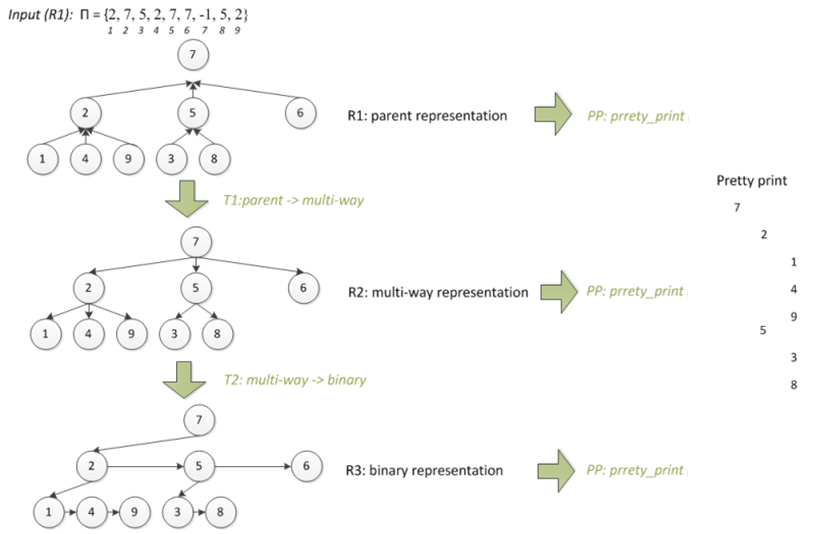
\includegraphics[width=\textwidth]{../Resources/lab6/Lab6_representations.png}

Analizați eficienta în timp și spațiu a celor două transformări. Ați
atins \emph{O(n)}? Ați folosit memorie adițională?

\end{document}